\section{Experiments}

% We systematically evaluate state-of-the-art language models on \benchmark to understand their embodied reasoning capabilities. Our experiments address three key questions: (1) How do current models perform across different types of embodied reasoning tasks? (2) What architectural properties enable or limit embodied reasoning? (3) How do environmental representations and training strategies affect performance?

We systematically evaluate current LLMs on \benchmark to assess their physical reasoning capabilities in embodied tasks. Our experiments examine: (1) How performance degrades when models must dynamically acquire tools and determine coordination requirements from task contexts, (2) Whether model scale and architectural choices affect constraint-based reasoning capabilities, and (3) How environmental information presentation and training approaches impact autonomous decision-making in embodied scenarios.

\subsection{Experimental Setup}

\paragraph{Model Selection.}
We evaluate nine representative models spanning three architectural paradigms. Closed-source models include GPT-4o \citep{hurst2024gpt} and Gemini-2.5-Flash \citep{comanici2025gemini}, representing current commercial state-of-the-art. Open-source foundation models cover a wide parameter range: Deepseek-V3 \citep{liu2024deepseek} at 671B parameters, the Qwen2.5 series \citep{team2024qwen2} at 3B, 7B, and 72B parameters, and Llama3.1-8B\citep{touvron2023llama}. This selection enables analysis of how model scale affects embodied reasoning. We also include reasoning-specialized models: Deepseek-R1 \citep{guo2025deepseek} and QwQ-32B\citep{li2024datacomp}, which employ explicit chain-of-thought reasoning during inference.

\paragraph{Evaluation Protocol.}
All models undergo identical evaluation to ensure fair comparison. We implement partial observability where agents must explore environments to discover object locations and properties, reflecting realistic deployment conditions. Each model completes 2,800 test scenarios across seven task categories with three independent runs for statistical reliability. We standardize prompts, environment descriptions, and action vocabularies across all models, with tool-dependent actions dynamically enabled based on context. This design ensures performance differences reflect reasoning capabilities rather than implementation artifacts. Detailed experimental configurations are provided in Appendix~\ref{sec:appendix_prompts}.

\paragraph{Fine-tuning Configuration.}
To assess whether supervised learning can address reasoning limitations, we fine-tune Qwen2.5-3B on expert trajectories. We collect 1,942 successful demonstrations from Qwen2.5-72B with complete environmental access, filtering for optimal action sequences. The resulting 20,346 instruction-action pairs train the model using standard causal language modeling objectives, testing whether smaller models can learn embodied reasoning patterns from larger models. Complete hyperparameters are listed in Appendix~\ref{sec:hyperparameters}.

\paragraph{Deployment Configurations.}
We evaluate models in two configurations. Single-agent scenarios test individual reasoning capabilities without collaborative complexity. Multi-agent scenarios employ centralized coordination where one model controls all agents with complete state visibility, isolating collaborative reasoning from communication challenges. This design choice allows us to assess pure multi-agent reasoning capabilities without confounding factors from limited observability or communication protocols.

\subsection{Main Results}
\begin{table*}[t]
\centering
\footnotesize  % Reduced from \small to fit better
\setlength{\tabcolsep}{3pt}  % Reduced from 4pt to save space
\begin{tabular*}{\textwidth}
{@{}l@{\extracolsep{\fill}}*{14}{c}@{}}
\toprule
\multirow{4}{*}{\textbf{Model}} & 
\multicolumn{8}{c}{\textbf{Single-Agent Tasks}} & 
\multicolumn{6}{c}{\textbf{Multi-Agent Tasks}} \\
\cmidrule(lr){2-9} \cmidrule(lr){10-15}
& \multicolumn{2}{c}{\textbf{Direct}} & \multicolumn{2}{c}{\textbf{Tool}} & \multicolumn{2}{c}{\textbf{Attribute}} & \multicolumn{2}{c}{\textbf{Compound}} & \multicolumn{2}{c}{\textbf{Explicit}} & \multicolumn{2}{c}{\textbf{Implicit}} & \multicolumn{2}{c}{\textbf{Compound}} \\
& \multicolumn{2}{c}{\textbf{Command}} & \multicolumn{2}{c}{\textbf{Use}} & \multicolumn{2}{c}{\textbf{Reasoning}} & \multicolumn{2}{c}{\textbf{Reasoning}} & \multicolumn{2}{c}{\textbf{Collab.}} & \multicolumn{2}{c}{\textbf{Collab.}} & \multicolumn{2}{c}{\textbf{Collab.}} \\
\cmidrule(lr){2-3} \cmidrule(lr){4-5} \cmidrule(lr){6-7} \cmidrule(lr){8-9} \cmidrule(lr){10-11} \cmidrule(lr){12-13} \cmidrule(lr){14-15}
& \textbf{SR} & \textbf{Step} & \textbf{SR} & \textbf{Step} & \textbf{SR} & \textbf{Step} & \textbf{SR} & \textbf{Step} & \textbf{SR} & \textbf{Step} & \textbf{SR} & \textbf{Step} & \textbf{SR} & \textbf{Step} \\
\midrule
\rowcolor{gray!20} \multicolumn{15}{@{}l@{}}{\textit{Closed-source Models}} \\
\midrule
GPT-4o & \underline{\textbf{96.6}} & 12.9 & 80.0 & 13.6 & \underline{\textbf{77.8}} & 12.3 & \textbf{69.2} & 14.5 & \textbf{90.0} & 13.9 & 77.5 & 14.4 & 32.0 & 22.9 \\
Gemini-2.5-Flash \xspace & 90.5 & 11.0 & \textbf{82.3} & 16.5 & 56.3 & 17.5 & 59.4 & 20.0 & 88.5 & 8.4 & \underline{\textbf{85.5}} & 7.1 & \textbf{40.5} & 16.2 \\
\midrule
\rowcolor{gray!20} \multicolumn{15}{@{}l@{}}{\textit{Reasoning-specialized Models}} \\
\midrule
Deepseek-R1 & \textbf{94.1} & 10.3 & \underline{\textbf{85.8}} & 14.1 & 41.9 & 12.2 & \underline{\textbf{70.6}} & 16.2 & \underline{\textbf{92.0}} & 7.4 & \textbf{84.5} & 9.6 & \underline{\textbf{48.5}} & 12.5 \\
QwQ-32B & 85.2 & 10.3 & 73.4 & 13.0 & \textbf{44.9} & 11.0 & 54.1 & 13.6 & 88.0 & 8.5 & 84.0 & 8.3 & 36.5 & 19.0 \\
\midrule
\rowcolor{gray!20} \multicolumn{15}{@{}l@{}}{\textit{Open-source Foundation Models}} \\
\midrule
Deepseek-V3 & \textbf{91.1} & 11.2 & \textbf{82.3} & 15.1 & 56.3 & 10.3 & \textbf{67.1} & 16.0 & \textbf{82.0} & 9.4 & 63.0 & 9.7 & \textbf{36.0} & 20.2 \\
Qwen2.5-72B & 89.7 & 14.7 & 56.4 & 21.7 & \textbf{57.4} & 17.2 & 66.7 & 21.1 & 56.0 & 24.1 & \textbf{65.4} & 15.6 & 28.6 & 29.5 \\
Llama3.1-8B & 24.9 & 34.4 & 8.3 & 34.6 & 9.9 & 34.8 & 12.4 & 34.3 & 4.0 & 3.5 & 1.5 & 2.1 & 0.0 & 3.4 \\
Qwen2.5-7B & 40.2 & 24.1 & 15.4 & 31.7 & 22.2 & 26.6 & 16.5 & 30.5 & 38.5 & 25.0 & 13.5 & 24.1 & 1.0 & 27.2 \\
Qwen2.5-3B & 0.6 & 30.5 & 1.8 & 31.3 & 0.6 & 34.0 & 2.9 & 32.9 & 8.5 & 20.4 & 1.5 & 16.3 & 0.5 & 16.8 \\
\quad + SFT & 76.3 & 15.4 & 45.0 & 24.7 & 33.5 & 22.8 & 36.5 & 24.7 & 22.5 & 29.2 & 5.5 & 28.3 & 1.0 & 27.1 \\
\bottomrule
\end{tabular*}
\caption{Performance across task categories. Success Rate (SR) measures task completion percentage, Step Count indicates average actions for successful completion. Bold indicates best in category, underline shows overall best.}
\label{tab:comprehensive_performance}
\end{table*}

Table~\ref{tab:comprehensive_performance} presents comprehensive evaluation results across our task hierarchy. The results reveal systematic performance patterns that validate our framework design and expose fundamental limitations in current models.

\begin{figure}[t]
    \centering
    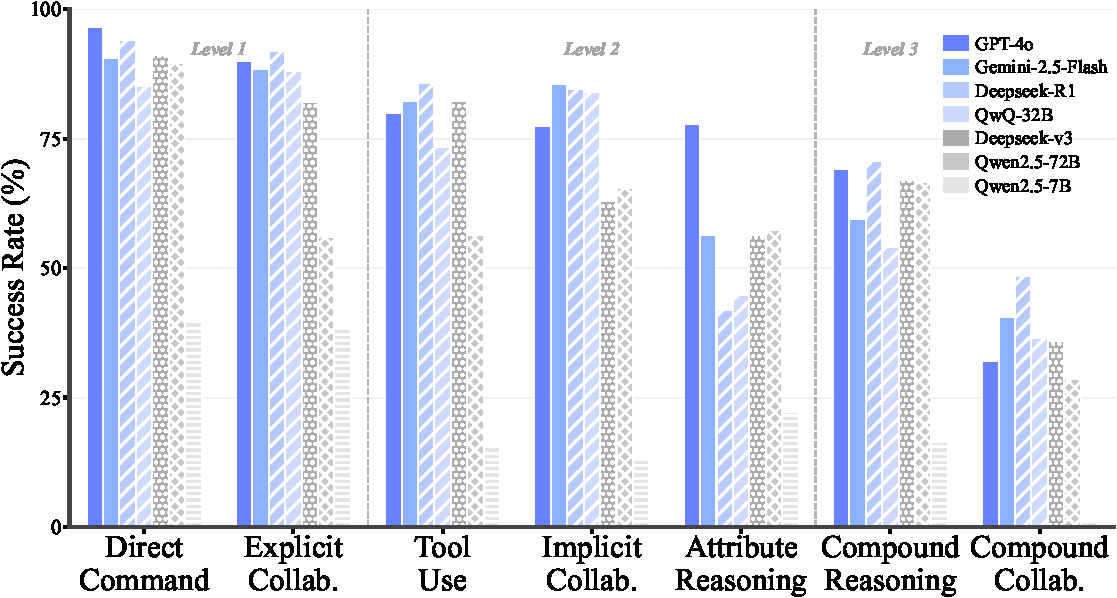
\includegraphics[width=0.75\columnwidth,clip]{figures/exp_1.pdf}
    \caption{Performance comparison across task categories demonstrating systematic difficulty hierarchy and distinct model performance tiers.}
    \label{fig:performance_comparison}
\end{figure}
\paragraph{Task Complexity Hierarchy.}
Figure~\ref{fig:performance_comparison} reveals systematic performance degradation across our task hierarchy, with success rates declining from 85.2-96.6\% on Direct Commands to 32.0-48.5\% on Compound Collaboration tasks. This consistent pattern confirms that performance differences reflect reasoning complexity rather than task difficulty alone. Tool Use (73.4-85.8\%) requires recognizing capability gaps from context, while Attribute Reasoning (41.9-77.8\%) demands grounding language in physical properties. Both involve inferring requirements from environmental constraints rather than following explicit instructions. Notably, Explicit Collaboration outperforms several single-agent tasks, indicating that reasoning about physical constraints poses greater challenges than multi-agent coordination when guidance is provided. The severe performance drop in compound tasks demonstrates that current models cannot integrate multiple constraints simultaneously, supporting our framework's focus on autonomous inference from physical context as the key determinant of embodied reasoning difficulty.


\paragraph{Model Scale and Reasoning Capabilities.}
\begin{figure}[t]
    \centering
    \begin{subfigure}[b]{0.48\textwidth}
        \centering
        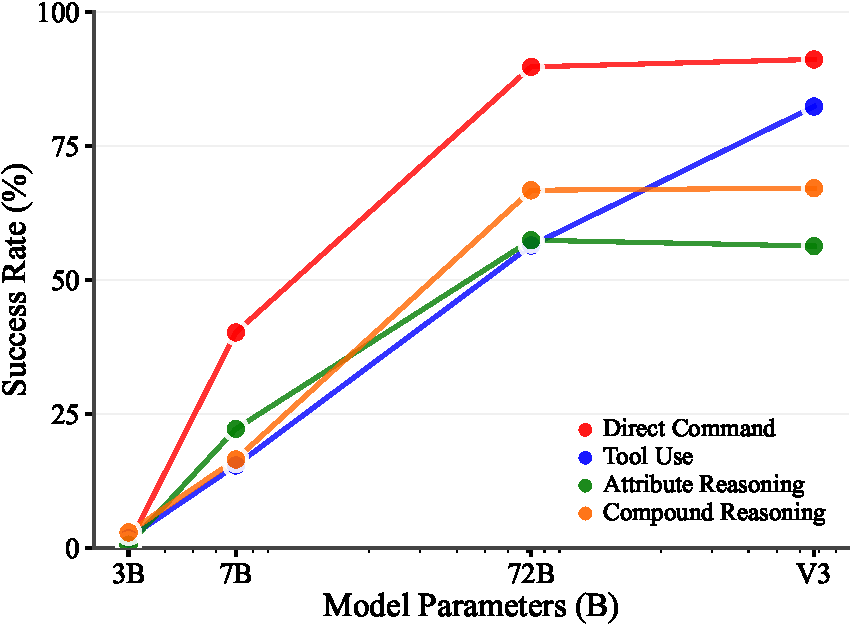
\includegraphics[width=\textwidth,clip]{figures/exp_2_parameter_scaling.pdf}
        \caption{Performance vs. model parameters.}
        \label{fig:parameter-scaling}
    \end{subfigure}
    \hfill
    \begin{subfigure}[b]{0.48\textwidth}
        \centering
        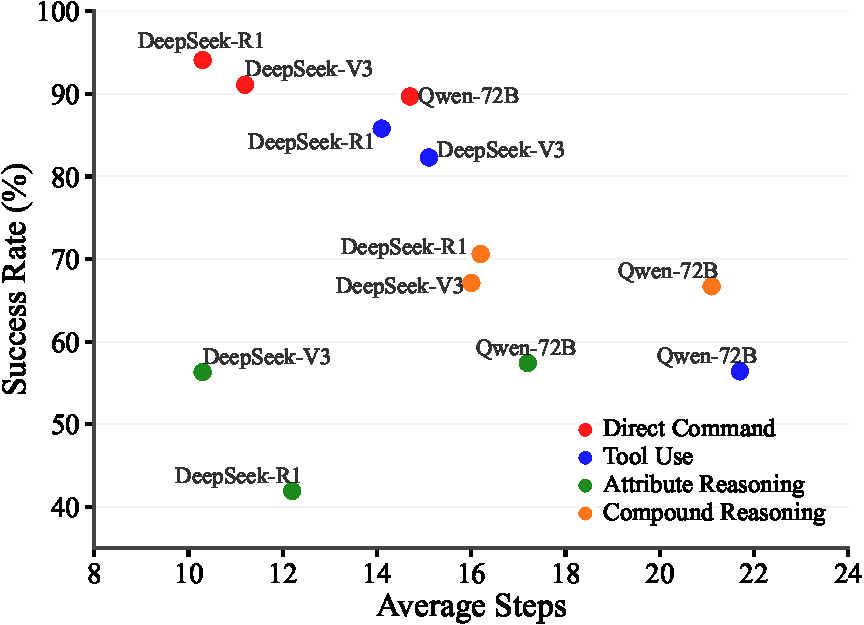
\includegraphics[width=\textwidth,clip]{figures/exp_2_step_efficiency.pdf}
        \caption{Success rate vs. execution steps.}
        \label{fig:step-efficiency}
    \end{subfigure}
    \caption{Scaling patterns reveal distinct thresholds for embodied reasoning capabilities. (a) Direct Command and Tool Use scale sharply with parameters while Attribute/Compound Reasoning plateau early. (b) Reasoning-specialized models achieve higher success through longer execution paths.}
    \label{fig:scaling-efficiency-analysis}
\end{figure}
\begin{figure}[t]
    \centering
    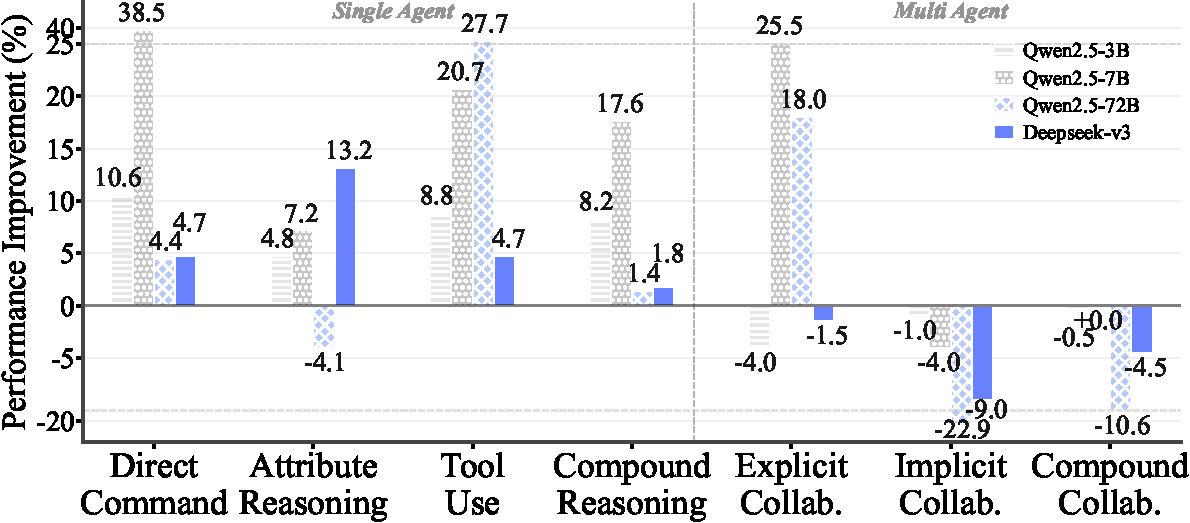
\includegraphics[width=0.75\columnwidth,clip]{figures/ae_1.pdf}
    \caption{Performance changes with World Graph enhancement. Tool Use and Attribute Reasoning benefit substantially, while Implicit Collaboration shows degradation, suggesting information overload effects.}
    \label{fig:global-observation-impact}
\end{figure}
Figure~\ref{fig:parameter-scaling} reveals distinct scaling patterns across task types. While Direct Command performance improves sharply with model size (from near-zero at 3B to over 90\% at 72B), tasks requiring physical constraint reasoning show more complex relationships. Tool Use exhibits similar steep scaling, suggesting that maintaining multi-step plans for capability acquisition correlates strongly with model capacity. However, Attribute Reasoning and Compound Reasoning plateau earlier, with diminishing returns beyond 72B parameters. This differential scaling indicates that raw parameter count enables better execution and planning but does not necessarily improve understanding of physical properties.

Table~\ref{tab:comprehensive_performance} provides further evidence distinguishing execution capability from genuine reasoning. Reasoning-specialized models like Deepseek-R1 achieve the highest performance on Compound Collaboration (48.5\%) despite lower scores on Attribute Reasoning (41.9\%) compared to GPT-4o (77.8\%). This performance inversion suggests these models excel at explicit logical planning but struggle with grounding abstract properties in physical contexts. The success rate versus step count trade-off in Figure~\ref{fig:step-efficiency} reinforces this interpretation: reasoning models achieve higher success through longer, more deliberate execution paths rather than efficient understanding of constraints. Fine-tuning results provide the clearest evidence that current models lack true embodied reasoning: while Qwen2.5-3B improves dramatically on single-agent tasks through imitation (0.6\% to 76.3\%), multi-agent performance remains negligible (1.5\% to 5.5\%), indicating that learned behaviors cannot generalize to scenarios requiring autonomous assessment of physical constraints and coordination needs.



\subsection{Detailed Analysis}
We conduct analyses to understand the factors driving model performance and identify specific capability bottlenecks.

\paragraph{Environmental Representation Impact.}
\begin{wraptable}{r}{0.52\textwidth}
\centering
\small
\setlength{\tabcolsep}{2pt}
\begin{tabular}{@{}lcc|cc|cc|cc@{}}
\toprule
\multirow{2}{*}{\textbf{Task}} & \multicolumn{2}{c|}{\textbf{3B}} & \multicolumn{2}{c|}{\textbf{7B}} & \multicolumn{2}{c|}{\textbf{72B}} & \multicolumn{2}{c}{\textbf{671B}} \\
\cmidrule{2-3} \cmidrule{4-5} \cmidrule{6-7} \cmidrule{8-9}
& w/o & w/ & w/o & w/ & w/o & w/ & w/o & w/ \\
\midrule
Direct Cmd & 0.6 & 11.2 & 40.2 & 78.7 & 89.7 & 94.1 & 91.1 & 95.9 \\
Tool Use & 1.8 & 10.7 & 15.4 & 36.1 & 56.4 & 84.0 & 82.3 & 87.0 \\
Attr. Reas. & 0.6 & 5.4 & 22.2 & 29.3 & 57.4 & 53.3 & 56.3 & 69.5 \\
Comp. Reas. & 2.9 & 11.2 & 16.5 & 34.1 & 64.5 & 65.9 & 67.1 & 68.8 \\
\midrule
Expl. Coll. & 8.5 & 4.5 & 38.5 & 64.0 & 62.5 & 80.5 & 82.0 & 80.5 \\
Impl. Coll. & 1.5 & 0.5 & 13.5 & 9.5 & 65.4 & 42.5 & 63.0 & 54.0 \\
Comp. Coll. & 0.5 & 0.0 & 1.0 & 1.0 & 28.6 & 18.0 & 36.0 & 31.5 \\
\bottomrule
\end{tabular}
\caption{Success rates (\%) with and without World Graph enhancement across model scales, revealing task-specific gains and unexpected drop in implicit collaboration.}
\label{tab:wg_results}
\end{wraptable}

% \begin{wrapfigure}{l}{0.5\textwidth}
%     \centering
%     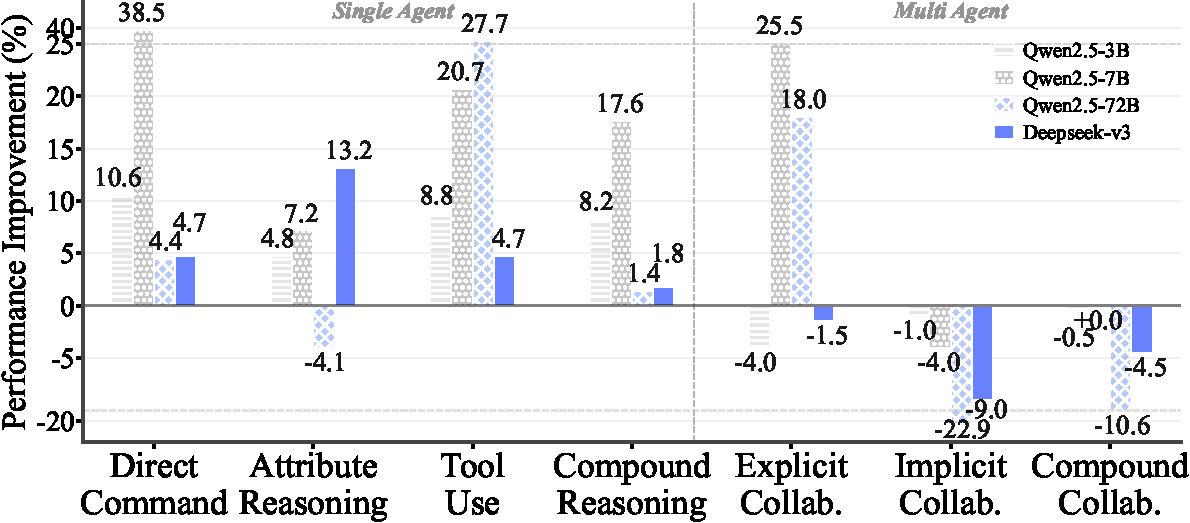
\includegraphics[width=0.48\textwidth,clip]{figures/ae_1.pdf}
%     \caption{Performance changes with World Graph enhancement. Tool Use and Attribute Reasoning benefit substantially, while Implicit Collaboration shows degradation, suggesting information overload effects.}
%     \label{fig:global-observation-impact}
% \end{wrapfigure}


Table~\ref{tab:wg_results} and Figure~\ref{fig:global-observation-impact} reveal task-specific effects of structured environmental knowledge. Tool Use benefits most significantly (up to 27.7\% improvement), as World Graph transforms spatial search into direct tool selection. Smaller models gain more than larger ones, suggesting that full environmental knowledge compensates for limited working memory. Conversely, Implicit Collaboration consistently drops with World Graph across all model scales. This counterintuitive pattern indicates that exploration-based discovery helps models focus on task-relevant constraints, while complete information introduces distraction. The divergent effects across task types demonstrate that optimal information presentation depends on reasoning requirements, not information quantity.

\paragraph{Computational Efficiency Trade-offs.}
\begin{figure}[htbp]
    \centering
    \begin{subfigure}[b]{0.48\textwidth}
        \centering
        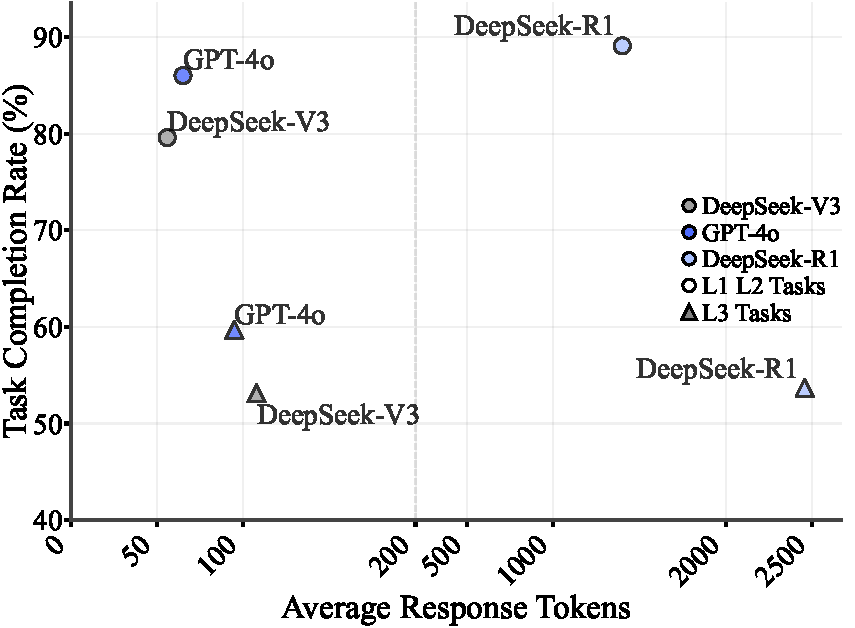
\includegraphics[width=\textwidth,clip]{figures/ae_3_efficiency_scatter.pdf}
        \caption{Resource utilization vs. success rate.}
        \label{fig:efficiency-analysis}
    \end{subfigure}
    \hfill
    \begin{subfigure}[b]{0.48\textwidth}
        \centering
        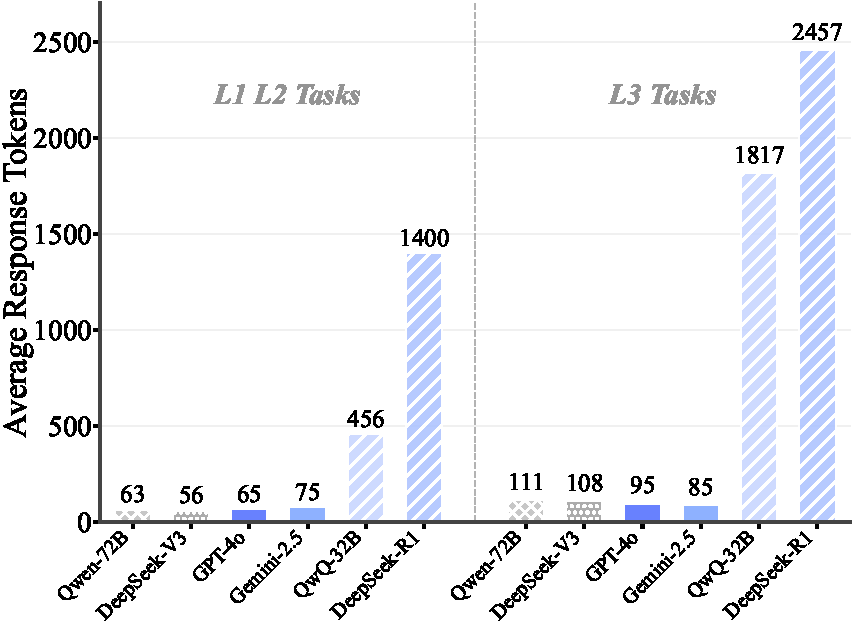
\includegraphics[width=\textwidth,clip]{figures/ae_3_token_consumption.pdf}
        \caption{Token consumption by model type.}
        \label{fig:token-consumption}
    \end{subfigure}
    \caption{Reasoning-specialized models achieve higher performance through increased computational overhead. (a) Efficiency-performance trade-offs across model architectures. (b) Token consumption patterns revealing computational costs of reasoning approaches.}
    \label{fig:combined-analysis}
\end{figure}

Figure~\ref{fig:efficiency-analysis} identifies three efficiency regimes with distinct cost-performance profiles. Foundation models achieve moderate performance with minimal tokens (456-1400), while commercial models trade higher token usage (1817-2457) for improved success rates. Reasoning models consume up to 12,000 tokens but excel on complex tasks. The efficiency frontier shifts dramatically between single and multi-agent scenarios: Gemini-2.5-Flash optimizes single-agent efficiency, but Deepseek-R1 becomes necessary for multi-agent tasks despite 75\% higher costs. This shift reflects the irreducible computational complexity of modeling multiple agent states and coordination protocols, suggesting no universal optimization exists across task types.

\paragraph{Execution Efficiency Analysis.}
\begin{figure}[htbp]
    \centering
    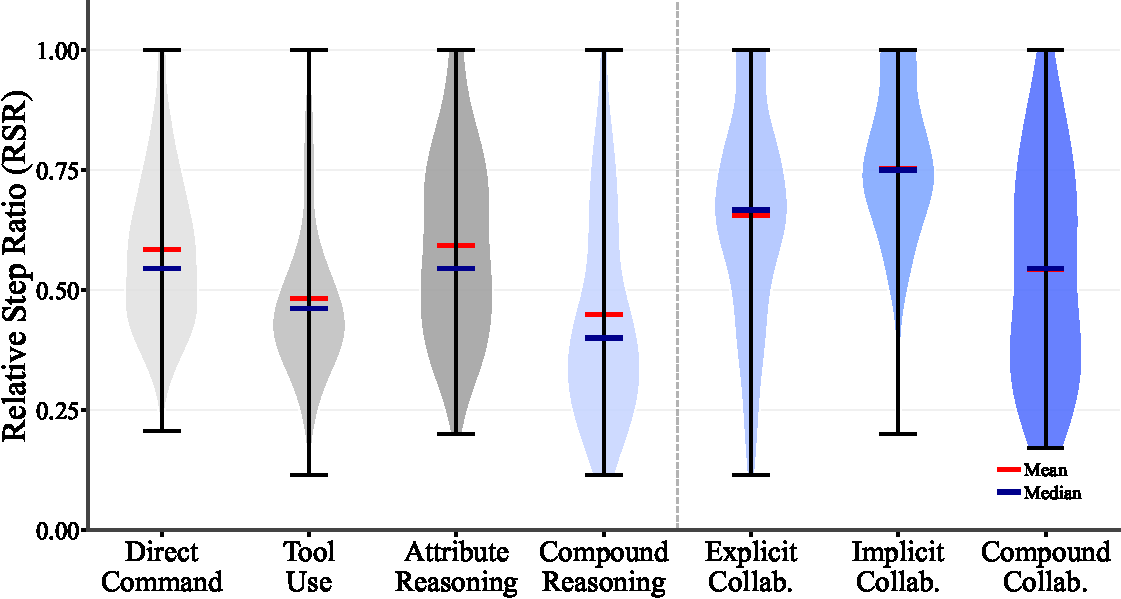
\includegraphics[width=0.75\columnwidth,clip]{figures/ae_2.pdf}
    \caption{Relative Step Ratio distributions showing execution efficiency compared to expert trajectories. Multi-agent tasks show both lower efficiency and higher variance than single-agent tasks.}
    \label{fig:expert-trajectory-efficiency}
\end{figure}
Figure~\ref{fig:expert-trajectory-efficiency} compares model solutions to expert demonstrations via Relative Step Ratios (RSR = $L_{\text{expert}}/L_{\text{model}}$). Single-agent tasks show consistent moderate efficiency (median RSR 0.40-0.55), while multi-agent tasks exhibit both lower efficiency and higher variance, reflecting uncertainty in coordination timing and strategy selection. Compound Collaboration reveals a striking bimodal distribution: models either adopt simple sequential execution or attempt complex parallel coordination, with no successful middle strategies. This polarization suggests current models lack adaptive coordination mechanisms, defaulting to extreme approaches rather than selecting strategies based on task constraints.